\documentclass[letter,11pt]{article}
\usepackage[utf8]{inputenc}
\usepackage{hyperref}
\usepackage{multicol}
\usepackage{wrapfig}
\usepackage{xcolor}
\usepackage{tabularx}

%====================
% OFFICIAL PUBLIC OVERLEAF TEMPLATE
% https://www.overleaf.com/latex/templates/data-science-tech-resume-template/zcdmpfxrzjhv
% 
%====================
%
% Resume template for data scientists, a complement to data-science-tech-cover-letter-template:
% https://www.overleaf.com/latex/templates/data-science-tech-cover-letter-template/gbrcqktbsfxf
%
% Files:        resume.tex: Main file
%               _header.tex: header code
%               TLCresume.sty: style file containing formatting details
%               section/objective: https://www.indeed.com/career-advice/resumes-cover-letters/resume-objective-examples
%               section/skills: table of skills
%               section/experience: projects or roles
%               section/education: schools and stuff
%               section/activities: optional, could comment out in resume.tex.
%
% Editor:       https://github.com/TimmyChan 
%               https://www.linkedin.com/in/timmy-l-chan/
%               
% Last Updated: March 24th, 2022
%
%====================


\usepackage{TLCresume}

%====================
% CONTACT INFORMATION
%====================
\def\name{Salim Mimouni, PhD} % Name Here
\def\phone{(+33) 659327018}
\def\city{\'{E}chirolles, Auvergne-Rh\^{o}ne-Alpes, France}
\def\email{salim.mimouni@gmail.com}
\def\LinkedIn{mimouni} % linkedin.com/in/______
\def\github{physics-programmer} % github username
\def\role{Data Scientist\\AI Orchestration \& Cloud--HPC Workflows} % JOB TITLE

%====================
% Header: Contact
%====================

\RequirePackage{fancyhdr}
\fancypagestyle{fancy}{%
\fancyhf{}
\lhead{%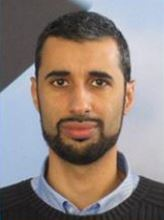
\includegraphics[width=2cm]{salim.jpg}
        
        \phone \\ % PHONE    
        \city \\ % city
	    \href{mailto:\email}{\email}} % EMAIL}
	\chead{%
	    \centering {\Huge \skills \name \vspace{.25em}} \\ % feel free to adjust vspace to 0 
	    {\color{highlight} \Large{\role}}}%
	    \rhead{ORCID: \href{https://orcid.org/0009-0008-7841-412X}{0009-0008-7841-412X}\\ % Portfolio
	    \href{https://github.com/\github}{github.com/\github} \\% Github
	    \href{https://www.linkedin.com/in/\LinkedIn}{linkedin.com/in/\LinkedIn}} % LinkedIn
\renewcommand{\headrulewidth}{1pt}% 2pt header rule
\renewcommand{\headrule}{\hbox to\headwidth{%
  \color{highlight}\leaders\hrule height \headrulewidth\hfill}}
}
\pagestyle{fancy}

\setlength{\headheight}{104pt}
\setlength{\headsep}{5pt}
%https://orcid.org/my-orcid?orcid=0009-0008-7841-412X

\begin{document}
%====================
% Objective Statement
%====================
\begin{wrapfigure}{l}{1.5cm}
    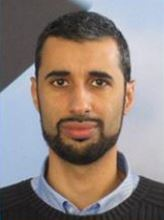
\includegraphics[width=1.5cm]{salim.jpg}
\end{wrapfigure}
% As a Data Scientist at Bull SAS, my expertise lies in developing robust data systems using Python OOP, Git, Docker, and MongoDB. My work has focused on multivariate time series processing and advanced machine learning techniques, utilizing tools such as scipy, sklearn, and tensorflow2/keras. I've been instrumental in High-Performance Computing (HPC) projects, optimizing workflows through Slurm and Optuna. My contributions include algorithm development in areas like image processing and recognition, driven by a commitment to continuous learning and collaborative problem-solving in a high-tech industry setting.

Data Scientist at Ryax Technologies, designing AI workflow orchestration for low-code platforms that deploy analytics and AI workflows across hybrid Cloud--HPC infrastructures. Current work spans multi-objective Kubernetes/Slurm scheduling, LLM-powered automation with agents and RAG pipelines, and transparent execution from Edge to Cloud to HPC. Five years at Bull built deep HPC expertise in recommendation systems, performance modeling, burst-buffer sizing, workflow optimization, production Python, multivariate time series, and scientific signal/image processing.

% As a Data Scientist, I have a solid background in Python OOP, classical Machine Learning tools, and some databases. My experience includes multivariate time series analysis and machine learning, utilizing tools like scipy, sklearn, and tensorflow2/keras. In my recent role at Bull SAS, I contributed to High-Performance Computing (HPC) projects, focusing on workflow optimization and HPC simulation, using tools such as Slurm and Optuna. My work also involves algorithm development in areas such as recognition and image processing. I am keen on continuous learning and collaboratively addressing new challenges.


% Accomplished Data Scientist with a keen interest in solving complex problems. Proficient in leveraging Python, Git, Docker, and MongoDB to create and manage efficient data systems. I have developed key skills in multivariate time series processing and machine learning, largely due to my consistent use of tools such as scipy, sklearn, and tensorflow2/keras. My background in scientific signal and image processing has provided a solid foundation for algorithm development involving recognition, alpha matting, classification, and segmentation. Recently, I have embarked on a journey to understand the nuances of High Performance Computing, using tools like slurm and nipype, and delving into data placement policies. As I continue to learn and grow in this field, I look forward to tackling new challenges and contributing to team successes.

% \blindtext[1]


\section{Skills}
% \begin{tabular}{p{11em} p{1em} p{43em}}
% \skills{Tools and Languages} & & Python, Scikit-learn, Pandas, Numpy, TensorFlow, Keras, Git, Docker, Django, MongoDB, Matlab\\

% \skills{Quantitative Research} & & Time series analysis, Machine learning, Deep Learning, Operational research, Reinforcement learning, Algorithm development, HPC simulation, Optuna, Wavelets, FFT, RCWA, NIRFAST, PMI, Data Modeling, Optimization\\

% \skills{Communication} & & English (professional), French (fluent), Arabic (mother tongue), Technical Communication, Cross-cultural Collaboration\\
% \end{tabular}

% \begin{tabularx}{\textwidth}{p{11em} p{1em} X}
% \skills{Tools and Languages} & & Python, Scikit-learn, Pandas, Numpy, TensorFlow, Keras, Git, Docker, Django, MongoDB, Matlab\\

% \skills{Quantitative Research} & & Time series analysis, Machine learning, Deep Learning, Operational research, Reinforcement learning, Algorithm development, HPC simulation, Optuna, Wavelets, FFT, RCWA, NIRFAST, PMI, Data Modeling, Optimization\\

% \skills{Communication} & & English (professional), French (fluent), Arabic (mother tongue), Technical Communication, Cross-cultural Collaboration\\
% \end{tabularx}

% \begin{tabularx}{\textwidth}{p{11em} p{1em} X}
% \skills{Tools and Languages} & & Proficient in Python, Scikit-learn, Pandas, Numpy; experienced in TensorFlow, Keras for deep learning; familiar with Git, Docker for version control and containerization; skilled in Django and MongoDB; proficient in Matlab for scientific computing.\\

% \skills{Quantitative Research} & & Specialized in time series analysis, clustering, classification and prediction for trading strategies, machine learning (ML) and deep learning (DL); operational research for solving real-world problems; reinforcement learning for adaptive decision-making; developed algorithms for HPC simulation and advanced modeling of application execution; adept in Optuna for hyperparameter tuning; utilized Wavelets, FFT for signal processing.\\

% \skills{Communication} & & Fluent in English (professional level), French (fluent speaker), and Arabic (mother tongue); effective in technical communication; experienced in cross-cultural collaboration and presenting complex concepts to diverse audiences.\\
% \end{tabularx}

\begin{tabularx}{\textwidth}{p{11em} p{1em} X}
\skills{Tools and Languages} & & Python, Git, Docker, Linux, SQL, MongoDB, PostgreSQL, REST/gRPC, RabbitMQ, CI/CD, Nix, Matlab.\\

\skills{Cloud, HPC \& AI} & & Kubernetes, Slurm, microservices, workflow orchestration, multi-objective scheduling, LLMs, agents, RAG, scikit-learn, TensorFlow/Keras, Optuna, time series, wavelets/FFT.\\

\skills{Certifications \& Languages} & & Deep Learning Specialization modules; Building Web Applications in Django. English (professional), French (native), Arabic (native).\\
\end{tabularx}



\section{Technical Experience}
\begin{multicols}{2}
%====================
% EXPERIENCE A
%====================
% \subsection{Data Scientist \hfill October 2019 --- Present}
% \subtext{Bull SAS\hfill Échirolles, Auvergne-Rhône-Alpes, France}
% \begin{zitemize}
% \item Led the development of a cutting-edge recommendation system for efficient data management in High-Performance Computing (HPC), utilizing advanced tools like slurm and nipype.
% \item Innovated a performance model-driven methodology for Burst Buffer sizing, significantly optimizing workflow duration and enhancing system efficiency.
% \item Executed complex multivariate time series preprocessing, embedding, clustering, and classification tasks, demonstrating proficiency in Python, Scikit-learn, Pandas, Numpy, TensorFlow, Keras, Git, Docker, Django, and MongoDB.
% \item Acquired extensive experience in HPC, Data Placement Policies, and crafting robust Python production code, underpinning a commitment to continuous learning and excellence in tackling challenging projects.
% \end{zitemize}


\subsection{Data Scientist \hfill September 2024 --- Present}
\subtext{Ryax Technologies\hfill Lyon, France}
% \begin{zitemize}
% \item Orchestrated the development of a state-of-the-art recommendation system for high-efficiency data management in High-Performance Computing (HPC) environments, utilizing advanced data science tools.
% \item Developed and implemented a novel, performance model-driven methodology for Burst Buffer sizing, dramatically enhancing workflow durations and overall system performance in HPC settings.
% \item Designed and built a simulation engine based on SimPy, integrating multiple machine learning components including application decomposers, workflow job dependency analyzers, and bandwidth sharing mechanisms to simulate application execution in an HPC simulated environment.
% \item Mastered complex multivariate time series preprocessing, embedding, clustering, and classification tasks, leveraging expertise in Python, Scikit-learn, Pandas, Numpy and MongoDB.
% \item Gained profound experience in High-Performance Computing, focusing on Data Placement Policies, and developed robust Python production code, demonstrating an unwavering commitment to continuous learning in challenging project environments.
% \end{zitemize}
\begin{zitemize}
\item AI workflow orchestration for hybrid Cloud--HPC deployments across Kubernetes and Slurm environments.
\item Orchestration algorithms for multi-site execution in Studio/Runner/Repository microservices.
\item LLM, agent, and RAG-driven automation pipelines with automated deployment and monitoring.
\item Multi-objective scheduling for cost, performance, privacy, autoscaling, bin packing, and GPU fractioning.
\end{zitemize}

\subsection{Data Scientist \hfill October 2019 --- May 2025}
\subtext{Bull (Atos)\hfill \'{E}chirolles, France}
\begin{zitemize}
\item Recommendation systems for efficient HPC data management; performance model-driven burst-buffer sizing and workflow optimization.
\item HPC environment: RHEL~7/8, Slurm, burst buffers, workflow managers (Nipype, Luigi).
\item Multivariate time-series preprocessing, embedding, clustering, and classification (scipy, sklearn, TensorFlow/Keras, Optuna).
\item Data placement policies: facility location, reinforcement learning, operations research, and production Python APIs.
\end{zitemize}

%====================
% EXPERIENCE B
%====================
\subsection{Maths and Physics Instructor \hfill September 2017 --- July 2019}
\subtext{Lycée Regnault Tanger (2017-2018), Lycée français Descartes de Rabat (2018-2019) \hfill Tanger, Morocco; Rabat, Morocco}
\begin{zitemize}
\item Taught mathematics and physics to students and prepared them for exams.
\end{zitemize}

%====================
% EXPERIENCE C
%====================
% \subsection{Image Processing Engineer \hfill May 2014 --- August 2017}
% \subtext{WiDisplay SARL \hfill Grenoble Area, France}
% \begin{zitemize}
% \item Pioneered algorithms in image/signal processing, enhancing machine learning and time series analysis.
% \item Streamlined image segmentation with fully convolutional network layers for precision object detection.
% \item Executed efficient data management and model deployment leveraging modern tools and cloud platforms.
% \end{zitemize}
\subsection{Image Processing Engineer \hfill May 2014 --- August 2017}
\subtext{WiDisplay SARL \hfill Grenoble Area, France}
\begin{zitemize}
\item Image/signal processing: recognition, alpha matting, segmentation, classification, and feature extraction.
\item ML/DL pipelines with TensorFlow/Keras, MatConvNet, Caffe, scikit-learn, statsmodels, and time-series models.
\item Data management and deployment using Pandas, NumPy, SQL/MongoDB, Docker, AWS, GCP, and Git.
\end{zitemize}

%====================
% EXPERIENCE D
%====================
\subsection{Nanoident Biometrics, CTO at SensCare \hfill March 2008 --- May 2014}
\subtext{Nanoident Biometrics SAS, SensCare SAS \hfill Grenoble, France}
\begin{zitemize}
\item Optical design and modeling for multimodal fingerprint and vein recognition devices.
\item Vein segmentation, fingerprint detection, optical/image preprocessing, and feature extraction.
\item ECG-like signal processing and cardiovascular-health modeling using FFT, wavelets, filtering, optical filtering, and video processing.
\item Technical leadership from proof-of-concept and experimentation to delivery.
\end{zitemize}
\end{multicols}

% %====================
% % EXPERIENCE A
% %====================
% \subsection{{ROLE / PROJECT A \hfill MMM YYYY --- Present}}
% \subtext{company A \hfill somewhere, state}
% \begin{zitemize}
% \item Lorem ipsum dolor sit amet, consectetur adipiscing elit.
% \item Suspendisse pretium elit quis ullamcorper ultricies.
% \item Morbi a nisl sit amet massa ultricies fermentum.
% \item Sed a diam et turpis tempor venenatis eget eget ipsum.
% \item Vestibulum fermentum justo vitae aliquet accumsan.
% \end{zitemize}

% %====================
% % EXPERIENCE B
% %====================
% \subsection{{ROLE / PROJECT B \hfill MMM YYYY --- MMM YYYY}}
% \subtext{company B \hfill somewhere, state}
% \begin{zitemize}
% \item Aenean semper felis et viverra eleifend.
% \item Integer aliquam odio id tellus sollicitudin, ut pellentesque elit blandit.
% \item Vestibulum iaculis quam ac nibh tincidunt rutrum.
% \end{zitemize}

% %====================
% % EXPERIENCE C
% %====================
% \subsection{{ROLE / PROJECT C \hfill MMM YYYY --- MMM YYYY}}
% \subtext{company C \hfill somewhere, state}
% \begin{zitemize}
% \item Donec volutpat turpis et placerat pharetra.
% \item Sed sit amet sem facilisis, scelerisque lectus aliquam, accumsan purus.
% \item Aliquam at urna congue dolor luctus sodales.
% \item Quisque vitae tortor at elit tincidunt molestie sed ac quam.
% \end{zitemize}

% %====================
% % EXPERIENCE D
% %====================
% \subsection{{ROLE / PROJECT D \hfill MMM YYYY --- MMM YYYY}}
% \subtext{company D \hfill somewhere, state}
% \begin{zitemize}
% \item Vestibulum accumsan massa quis dignissim faucibus.
% \item Maecenas suscipit mi ut ullamcorper pharetra.
% \item In vitae ligula tristique, iaculis tortor in, egestas magna.
% \item In fringilla purus malesuada lectus imperdiet pulvinar.
% \item Nulla eu dolor congue, mollis dui a, eleifend purus.
% \end{zitemize}

% %====================
% % EXPERIENCE E
% %====================
% %\subsection{{ROLE / PROJECT E \hfill MMM YYYY --- MMM YYYY}}
% %\subtext{company E \hfill somewhere, state}
% %\begin{zitemize}
% %\item In lobortis libero consectetur eros vehicula, vel pellentesque quam fringilla.
% %\item Ut malesuada purus at mi placerat dapibus.
% %\item Suspendisse finibus massa eu nisi dictum, a imperdiet tellus convallis.
% %\item Nam feugiat erat vestibulum lacus feugiat, efficitur gravida nunc imperdiet.
% %\item Morbi porta lacus vitae augue luctus, a rhoncus est sagittis.
% %\end{zitemize}


\newpage

\section{Education}
% \skills{PhD in Physics}, \textit{Université Grenoble Alpes}, \href{https://theses.hal.science/tel-00493016/document}{\textit{High-Density Near-Field Optical Disc Recording}} (Doctoral dissertation) \hfill November 2004 - November 2007

% \skills{Engineer's Diploma}, \textit{Ecole Supérieure d'Optique - Institut d'Optique Graduate School} \hfill 2001 - 2004

% %\skills{Research Master Degree in Physics: matter-wave interactions}, \textit{Paris-Sud University (Paris XI)} \hfill 2003 - 2004
% \skills{Research Master Degree in Physics: matter-wave interactions}, \textit{Paris-Sud University (Paris XI)}, \href{https://www.researchgate.net/profile/C-Lepers/publication/237587056_AMELIORATION_DE_LA_SENSIBILITE_D%27UN_DISPOSITIF_OLCR_PAR_INTERPOLATION_RECADRAGE_ET_SOMMATION_D%27INTERFEROGRAMMES/links/00b7d53c53c4232e86000000/AMELIORATION-DE-LA-SENSIBILITE-DUN-DISPOSITIF-OLCR-PAR-INTERPOLATION-RECADRAGE-ET-SOMMATION-DINTERFEROGRAMMES.pdf}{\textit{Improving the sensitivity of an OLCR device by interpolation, recentering and summing interferograms}} \hfill 2003 - 2004

% \skills{Intensive two-year undergraduate course in Mathematics and Physics}, \textit{CPGE Joffre, PCSI, PC*} \hfill 1999 - 2001


\begin{multicols}{2}

\skills{PhD in Physics}, \textit{Université Grenoble Alpes}, \href{https://theses.hal.science/tel-00493016/document}{\textit{High-Density Near-Field Optical Disc Recording}} (Doctoral dissertation) \hfill November 2004 - November 2007
\begin{itemize}
\item Focused on breakthrough research in Near-Field High Density Optical Data Storage.
\item Designed innovative super-resolving optical heads for data storage, including new solid immersion lens and plasmonics components.
\item Demonstrated an experimental system capable of recording/reading 1.5 Terabytes on a single 12cm diameter optical disk, surpassing traditional resolution limits.
\item Filed five patents based on the new system architecture and experimental proof of concept.
\end{itemize}

\skills{Engineer's Diploma}, \textit{Ecole Supérieure d'Optique - Institut d’Optique Graduate School} \hfill 2001 - 2004
\begin{itemize}
\item Specialized in Optics and Photonics, with a focus on signal and image processing.
\item Gained comprehensive knowledge in advanced optics technologies and applications.
\end{itemize}

\skills{Research Master Degree in Physics: matter-wave interactions}, \textit{Paris-Sud University (Paris XI)}, \href{https://www.researchgate.net/profile/C-Lepers/publication/237587056_AMELIORATION_DE_LA_SENSIBILITE_D%27UN_DISPOSITIF_OLCR_PAR_INTERPOLATION_RECADRAGE_ET_SOMMATION_D%27INTERFEROGRAMMES/links/00b7d53c53c4232e86000000/AMELIORATION-DE-LA-SENSIBILITE-DUN-DISPOSITIF-OLCR-PAR-INTERPOLATION-RECADRAGE-ET-SOMMATION-DINTERFEROGRAMMES.pdf}{\textit{Improving the sensitivity of an OLCR device by interpolation, recentering and summing interferograms}} \hfill 2003 - 2004
\begin{itemize}
\item Conducted in-depth research on enhancing the sensitivity of Optical Low Coherence Reflectometry (OLCR) devices.
\item Developed and validated a new method for improving OLCR measurements.
\end{itemize}

\skills{Intensive two-year undergraduate course in Mathematics and Physics}, \textit{CPGE Joffre, PCSI, PC*} \hfill 1999 - 2001
\begin{itemize}
\item Completed a rigorous preparatory program in Mathematics and Physics, laying a solid foundation for advanced studies in Physics.
\end{itemize}


\end{multicols}

% make a newpage wherever it is a clean break
% \newpage

\section{Patents \& publications}

%\section*{Patents}

% \begin{itemize}
% \item \href{https://patents.google.com/patent/EP3989074A1/en}{Method for optimizing execution of high-performance computing workflows}, P. Couvée, S. Mimouni, S. Robert, L. Vincent, Patent No. EP-3989074-A1, April 2022.
% \item \href{https://patents.google.com/patent/WO2011026986A1/en}{An optical device for sensing a plethysmographic signal using a matrix imager}, S. Mimouni, Patent No. WO-2011026986-A1, March 2011.
% \item \href{https://patents.google.com/patent/JP2010092581A/en}{Test device for determining characteristics of material used for optical storage}, S. Mimouni, F. Laulagnet, Patent No. JP-2010092581-A, April 2010.
% \item \href{https://patents.google.com/patent/EP2297745A1/fr}{Dispositif de piégeage de particules}, D. Neel, S. Getin, B. HYOT, S. Mimouni, Patent No. EP-2297745-A1, March 2011.
% \item \href{https://patents.google.com/patent/WO2009037249A1/fr}{Lentille a immersion solide et procede de realisation associe}, M. BRUN, S. Mimouni, S. Nicoletti, L. Poupinet, H. Moriceau, Patent No. WO-2009037249-A1, March 2009.
% \item \href{https://patents.google.com/patent/WO2008135485A1/fr}{Procede et systeme de lecture d'informations optiques a haute densite}, S. Mimouni, F. Laulagnet, Patent No. WO-2008135485-A1, November 2008.
% \item \href{https://patents.google.com/patent/WO2007144313A1/fr}{Composant optique fonctionnant en transmission en champ proche}, S. Mimouni, L. Poupinet, Patent No. WO-2007144313-A1, December 2007.
% \item \href{https://patents.google.com/patent/EP2002436B1/fr}{Lentille a immersion solide a capacite de focalisation accrue.}, S. Mimouni, Patent No. EP-2002436-B1, November 2009.
% \item \href{https://ieeexplore.ieee.org/abstract/document/1632720}{Polarization States in Near-Field Optical Recording System using a Solid Immersion Lens Illuminated by a Coherent Polarized Light}, S. Mimouni, L. Poupinet and P. Chaton, 2006 Optical Data Storage Topical Meeting, Montreal, QC, Canada, 2006, pp. 64-66.
% \end{itemize}

\begin{multicols}{2}
{\small
\begin{itemize}
\item \href{https://doi.org/10.1016/j.future.2025.108034}{I/O patterns modeling of HPC applications with call stacks for predictive prefetch}, Future Generation Computer Systems, 2026.
\item \href{https://doi.org/10.1145/3733723.3733745}{Investigating the Use of File Advisory Hints on Lustre and GPFS}, SSDBM, 2025.
\item \href{https://doi.org/10.1145/3719330.3721227}{Characterizing the use of DVFS for HPC I/O optimization}, EuroSys Workshop, 2025.
\item \href{https://doi.org/10.1145/3624062.3624189}{GrIOt: Graph-based Modeling of HPC Application I/O Call Stacks for Predictive Prefetch}, SC Workshops, 2023.
\item \href{https://patents.google.com/patent/EP3989074A1/en}{Method for optimizing execution of high-performance computing workflows}, P. Couvée, S. Mimouni, S. Robert, L. Vincent, European Patent No. EP3989074A1, 2022.
\item \href{https://patents.google.com/patent/WO2011026986A1/en}{An optical device for sensing a plethysmographic signal using a matrix imager}, S. Mimouni, Patent No. WO2011026986A1, 2011.
\item \href{https://patents.google.com/patent/WO2008135485A1/fr}{Procede et systeme de lecture d'informations optiques a haute densite}, S. Mimouni, F. Laulagnet, Patent No. WO2008135485A1, 2010.
\item \href{https://patents.google.com/patent/WO2007144313A1/fr}{Composant optique fonctionnant en transmission en champ proche}, S. Mimouni, L. Poupinet, Patent No. WO2007144313A1, 2007.
\item Full research profile: \href{https://orcid.org/0009-0008-7841-412X}{orcid.org/0009-0008-7841-412X}.
\end{itemize}
}
\end{multicols}

% \begin{tabular}{lll}
% \textbf{Title} & \textbf{Authors} & \textbf{Details} \\
% \href{https://patents.google.com/patent/EP3989074A1/en}{Method for optimizing execution...} & P. Couvée, S. Mimouni, S. Robert, L. Vincent & Patent No. EP-3989074-A1, April 2022 \\
% \href{https://patents.google.com/patent/WO2011026986A1/en}{An optical device for sensing...} & S. Mimouni & Patent No. WO-2011026986-A1, March 2011 \\
% \href{https://patents.google.com/patent/JP2010092581A/en}{Test device for determining characteristics...} & S. Mimouni, F. Laulagnet & Patent No. JP-2010092581-A, April 2010 \\
% \href{https://patents.google.com/patent/EP2297745A1/fr}{Dispositif de piégeage de particules} & D. Neel, S. Getin, B. HYOT, S. Mimouni & Patent No. EP-2297745-A1, March 2011 \\
% \href{https://patents.google.com/patent/WO2009037249A1/fr}{Lentille a immersion solide...} & M. BRUN, S. Mimouni, S. Nicoletti, L. Poupinet, H. Moriceau & Patent No. WO-2009037249-A1, March 2009 \\
% \href{https://patents.google.com/patent/WO2008135485A1/fr}{Procede et systeme de lecture...} & S. Mimouni, F. Laulagnet & Patent No. WO-2008135485-A1, November 2008 \\
% \href{https://patents.google.com/patent/WO2007144313A1/fr}{Composant optique fonctionnant...} & S. Mimouni, L. Poupinet & Patent No. WO-2007144313-A1, December 2007 \\
% \href{https://patents.google.com/patent/EP2002436B1/fr}{Lentille a immersion solide...} & S. Mimouni & Patent No. EP-2002436-B1, November 2009 \\
% \href{https://ieeexplore.ieee.org/abstract/document/1632720}{Polarization States in Near-Field...} & S. Mimouni, L. Poupinet and P. Chaton & 2006 Optical Data Storage Topical Meeting, Montreal, QC, Canada, 2006, pp. 64-66 \\
% \end{tabular}





\end{document}
